% *****************************************************************************
%
% Author: Léonard Binet
%
% Professional thesis report.
%
% *****************************************************************************


\documentclass[a4paper, 12pt]{report}

\usepackage{geometry}
\usepackage[english]{babel}
\usepackage[utf8]{inputenc}
\usepackage[T1]{fontenc}
%\usepackage{graphicx}
%\usepackage[pdftex]{graphicx}
\usepackage{setspace}
\usepackage[pdftex]{hyperref}
\usepackage{amsmath,amsthm,amsfonts,amssymb}
\usepackage[T1]{fontenc}
\usepackage{multirow}
\usepackage{svg}
\usepackage{float}
\usepackage{textcomp}
\usepackage{fullpage}
\usepackage{fancyvrb}
\usepackage{fancyhdr}
\usepackage{lmodern}
\usepackage{sistyle}
% \usepackage{color}
\usepackage{xcolor}
\usepackage{float}
\usepackage{wrapfig}
\usepackage[justification=centering, font={small}]{caption}
\usepackage{verbdef}
\usepackage{dsfont}
\usepackage[normalem]{ulem}
\usepackage{amssymb} % for mathbb
\usepackage{outlines}

% for diagrams
\usepackage{tikz}
\usetikzlibrary{shapes,arrows, positioning}

% force footnotes to be on the bottom
\usepackage[bottom]{footmisc}

% for tables
\usepackage{booktabs}
\usepackage{tabularx,ragged2e}
\newcolumntype{L}{>{\arraybackslash}X}

% for pseudocode
\usepackage{algorithm}
\usepackage{algorithmic}
% \usepackage[noend]{algpseudocode}

% bigger operators
\usepackage{relsize}

% neural figures
\usepackage{tikz}
\def\layersep{2.5cm}


% for cases
\makeatletter
\renewcommand{\env@cases}[1][@{}l@{\quad}l@{}]{%
  \let\@ifnextchar\new@ifnextchar
  \left\lbrace
  \def\arraystretch{1.2}%
  \array{#1}%
}
\makeatother

% Remove indent of 2nd paragraph in sections, subsections, etc.
% Uncomment to enable
\setlength{\parindent}{0pt}

\newcommand\Framing[1]
  { \hspace{10mm}
     \framebox{#1}\hspace{10mm}}

% nested bullet lists
\renewcommand{\labelitemii}{$\star$}

% -----------------------------------------------------------------
%                              Tools
% -----------------------------------------------------------------

% Adding source to figures
\newcommand*{\captionsource}[2]{%
  \caption[{#1}]{%
    #1%
    \\\hspace{\linewidth}%
    \textbf{Source:} #2%
  }%
}
% Format multiline text in subscripts
\newcommand\multiLine[1]{\text{\scriptsize\tabular[t]{@{}l@{}}#1\endtabular}}

\newcommand{\reporttitle}{Product Attribute prediction}     % Titre
\newcommand{\reportauthor}{} % Auteur
\newcommand{\reportsubject}{Professional Thesis} % Sujet
\newcommand{\HRule}{\rule{\linewidth}{0.5mm}}
\setlength{\parskip}{1ex} % Espace entre les paragraphes

% indent a paragraph
\newenvironment{myindentpar}[1]%
 {\begin{list}{}%
         {\setlength{\leftmargin}{#1}}%
         \item[]%
 }
 {\end{list}}

% -----------------------------------------------------------------

\geometry{top=2.5cm,left=2.6cm,right=2.6cm,bottom=2.5cm,headsep=1cm}
\hypersetup{pdfborder={0 0 0},
colorlinks,urlcolor=blue,linkcolor=blue,citecolor=blue,filecolor=blue,
pdftitle=
}


\begin{document}

\pagestyle{fancy}
\fancyhead[C]{Léonard\, Binet}
\fancyhead[R]{Telecom ParisTech}
\fancyhead[L]{Alkemics}

\cfoot{\thepage}
\setlength\headheight{15pt}

% Inspiré de http://en.wikibooks.org/wiki/LaTeX/Title_Creation

\begin{titlepage}

\begin{center}

\begin{center}
    
\includegraphics[height=3cm]{images/logo-telecom-paristech.png}
    \hspace{\stretch{1}}
    
\includegraphics[width=6cm]{images/Logo-Alkemics.png}
\end{center}

\vspace{160pt}

\textsc{\Large \reportsubject}\\[0.5cm]
\HRule \\[0.4cm]
{\huge \bfseries \reporttitle}\\[0.4cm]
\HRule \\[1.5cm]

\vspace{50pt}

 \large{\textbf{Léonard Binet} \\ Telecom ParisTech \\ Post-Master's Degree \\ BGD \\ \vspace{0.25cm} - \vspace{0.25cm} \\
  Company supervisor: Pierre Arbelet \\ Academic supervisor: Slim Essid}

\vfill

{\large January 01, 2018}

\end{center}

\end{titlepage}

\begin{abstract}

Confronted with challenges concerning product data quality, Alkemics decided to explore new ways to provide value proposition to its clients.

This paper aims at explaining how we tackled data-quality challenges at Alkemics, with the use of some machine learning algorithms.
But rather than solely describing models and algorithms, a focus is put on implementation and business added value. 


\end{abstract}


\cleardoublepage   % Dans le cas du recto verso, ajoute une page blanche si besoin
\tableofcontents % Table des matières
\sloppy            % Justification moins stricte : des mots ne dépasseront pas des paragraphes
%\cleardoublepage

\cleardoublepage
\chapter{Introduction}

Alkemics is a start-up that was founded in 2011. Back then, they created e-merchandising tools to improve user experience on e-commerce websites. It then evolved to become a platform that enables the FMCG (Fast-Moving Consumer Goods) ecosystem to share all their data, from product to transactional information, in order to improve pricing, supply, marketing.

Alkemics develops products that enable collaboration between Brands and Retailers, and tackle the challenges of omni-channel commerce and smart customer interaction.

\section{Alkemics}

\begin{figure}[H]
\centering
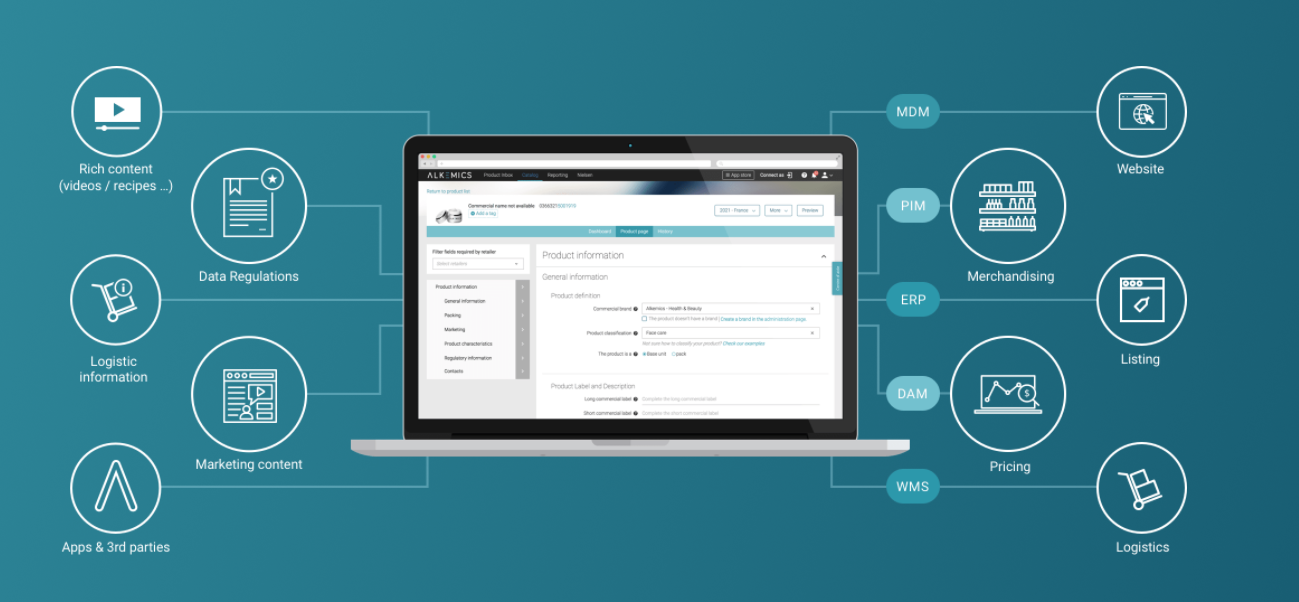
\includegraphics[scale=0.30]{./images/alkemics_website_global.png}
\caption{Alkemics}
\end{figure}

\subsection{Product Data Empowerment}

Because of increasing regulations, new customer demands, omni-channel communications, there is a growing need for richer and more exhaustive product information as well as an exponentially growing number of products. Some products change more than 10 times per year (promotion, seasonality, new recipes, new packagings...), and overall, 40\% of products are renewed every year.

This cascades in a series of problems that handicap manufacturers, retailers and consumers: logistics struggle to maintain stock, accounting systems fail to track how different products are actually the same consumption unit, pricing teams struggle to maintain price coherency in this dynamic environment, marketing teams are inefficient to share richer and richer content about the product, BI teams feel that the consumption of the consumer are changing while they actually don't.

This problem is called product chaining. It describes the ability to connect products that share a given set of attributes in order to understand how they relate.

To overcome these problems, Alkemics built a product taxonomy reinforced by an ontology. PDE \footnote{Product Data Empowerment} team is fully dedicated to enhance the classification task to automatically classify the category of products, as well as the brand and other attributes such as the packaging or the price range. The classification task mainly uses Natural Language Processing techniques and distances in semantic spaces. PDE is also in charge of the management of the product data model.


\subsection{Product Stream}

Product Stream is a web application that enables:
\\

\textbf{Makers} to:
    \begin{itemize}
    \item Collect product information from all the stakeholders of the organization: the \textit{supply team} who knows the size and weight of the product, the \textit{marketing team} who owns the pictures, videos as well as the brand content, the \textit{quality team} who masters the composition, nutritional values, etc.
    \item Store product information in a centralized way, so everyone in the organization can have access to it (DAM \footnote{Digital Asset Management}).
    \item Distribute product information so every partner has the same up-to-date information. This includes retailers, but also marketing agencies, trade marketing agencies, ... (EDI \footnote{Electronic Data Interchange} / PIM \footnote{Product information management})
    \item Collaborate with 3rd parties to collect user reviews,  receive data quality reports,  print coupons, use buy-it-now solutions.
    \end{itemize}

\textbf{Retailers} to:
    \begin{itemize}
    \item Have access to best-in-class product information to power their tools and feed their digital supports (EDI)
    \item Collaborate with manufacturers to reference new products \& innovations, run call-for-proposals for promotional formats, etc…
    \item Connect products that share a given set of attributes in order to understand how they relate (Product Chaining).
    \end{itemize}

\subsection{The technological stack}

\textbf{Micro-services architecture}
The stack in Alkemics is composed of set of dozens of micro services communicating with synchronous calls (HTTPS) and both synchronous and asynchronous messaging (TCP enabled by Rabbit MQ).
Each service has a domain specific task: data ingestion, data classification, APIs for merchandising, etc. A subset of the services are exposed to third parties and clients.

\textbf{User interface}
User Interface dashboards also call the APIs to make functionalities available to the users (makers and retailers) trough a web browser.
The front part of the website is implemented with React framework.

\textbf{APIs and SDKs}
A set of SDKs are also provided to retailers to allow them to use merchandising functionalities directly embedded in their websites.

\textbf{Storage vs indexation}
All Alkemics crucial data is stored in relational databases (MySQL). Yet if relationnal databases provide very useful functionalities to guaranty integrity of data, its indexing capabilities remain quite poor in comparison to non-relational databases.

That's we also create ElasticSearch indexes, containing data that is already stored in relational databases, but indexed in a format allowing quick and performant queries.


\section{Professional thesis objective}

This professional thesis aims at implementing machine learning techniques to improve products data quality.

%\cleardoublepage
\include{p_fasttext}
%\cleardoublepage
%\chapter{Development} % (fold)
\label{cha:development}


\section{Workflow} % (fold)
\label{sec:workflow}


% subsection features_distributions (end)

% chapter development (end)

%\cleardoublepage
%\chapter{Results} % (fold)
\label{cha:results}

\section{Classification} % (fold)
\label{sec:classification}

% subsection scalability (end)

% section to_go_further (end)

% chapter results (end)

\cleardoublepage
%\chapter{Parallel tasks} % (fold)
\label{cha:parallel_tasks}


% chapter parallel_tasks (end)

%\cleardoublepage
%\chapter*{Conclusion} % (fold)
\addcontentsline{toc}{chapter}{Conclusion}
\label{cha:conclusion}


During this project, we transformed a workflow dedicated to one multiclass field, to a much flexible and adaptable workflow.


Machine learning hype drives attention mostly to models and algorithms. 
Yet, this project convinced me that 90\% of a project success depends on pragmatism and implementation.

Fields to explore ....

Lot more to say when paper will be finished.

\chapter*{Acknowledgment}

Big up to @caillou for ML, and Alkemics as a whole for engineering skills.
Big up to MS BGD @Telecom for accepting me in 2017 promo

\addcontentsline{toc}{chapter}{Acknowledgment}

%\cleardoublepage
\appendix
\chapter{Logistic Regression: from binary, to multiclass, to multilabel} % (fold)
\label{cha:multilabel_classification}


\section*{Common notations}


\subsection*{Notations for single-labeled samples}

\subsubsection*{Probabilistic notations}

\begin{outline}
\1 X random vector, $\mathcal{X} \subset \mathbb{R}^d$
\begin{align}
	X = \left[
	\begin{array}{cccc}
		X_{1} \\
		X_{2} \\
		\vdots\\
		X_{d} \\
	\end{array}\right]
\end{align}

\1 Y discrete random variable, $\mathcal{Y} $, with $|\mathcal{Y}|$ finite. In practice, Y is encoded as an integer, ie $\mathcal{Y} \subset \mathbb{N} $ and $Y \in \mathbb{N}$

\1 P joint probability of X and Y $(X,Y)$ (unknown).
\end{outline}

\subsubsection*{Empirical notations}

\begin{outline}
\1 $x$, a vector sample, which is a realization of X (the empirical counterpart of X) $x \in \mathbb{R}^d$:
\begin{align}
	x = \left[
	\begin{array}{cccc}
		x_{1} \\
		x_{2} \\
		\vdots\\
		x_{d} \\
	\end{array}\right]
\end{align}

\1 $y$, a sample, which is a realization of Y (the empirical counterpart of Y): $y \in \mathcal{Y} \subset \mathbb{N}$

\1 $ \mathcal{D}_m = \{(x^{(i)}, y^{(i)}), i \in 1,m\} \in (\mathcal{X},\mathcal{Y})^m$ a learning set containing $m$ samples $iid$ and from P.\\
\end{outline}

Note:
For the $i^{th}$ sample, $x^{(i)}$ $y^{(i)}$, which are vectors, we'll respectively denote the $j^{th}$ component as follow: $x_j^{(i)}$ and $y_j^{(i)}$


\subsection*{Notations for multi-labeled samples}

Everything is the same except that labels are no longer scalars but vectors, with $K = |\mathcal{Y}|$:

\begin{outline}
\1 Y random vector, $\mathcal{Y} \subset \mathbb{N}^d$
\begin{align}
	Y = \left[
	\begin{array}{cccc}
		Y_{1} \\
		Y_{2} \\
		\vdots\\
		Y_{K} \\
	\end{array}\right]
\end{align}

\1 Y discrete random variable, $\mathcal{Y} $, with $|\mathcal{Y}|$ finite. In practice, Y is encoded as an integer, ie $\mathcal{Y} \subset \mathbb{N} $ and $Y \in \mathbb{N}$

\1 P joint probability of X and Y $(X,Y)$ (unknown).
\end{outline}






\section{Binary case: Logistic regression} % (fold)
\label{sec:workflow}


We want to predict the value of $y^{(i)}$ for the example $x^{(i)}$ using a function $y = h_\theta(x) $ with binary-valued labels $\left(y^{(i)} \in \{0,1\}\right)$. We want to predict the probability that a given example belongs to the “1” class versus the probability that it belongs to the “0” class. Specifically, we will try to learn a function of the form:

\subsection{Model}
\begin{align}
	P(Y=1|X=x) &= f_\theta(x) \\
			   &= \frac{1}{1 + \exp(-\theta^\top x)} \\
			   &= \sigma(\theta^\top x),\\
	P(Y=0|X=x) &= 1 - f_\theta(x) \\
			   &= \sigma(-\theta^\top x)
\end{align}

With:
\begin{align}
	\sigma(z) \equiv \frac{1}{1 + \exp(-z)}
\end{align}

the “logistic” function. It is an S-shaped function that “squashes” the value of $\theta^\top x$ into the range [0, 1] so that we may interpret $f_\theta(x)$ as a probability. 

Our goal is to search for a value of $\theta$ so that the probability $P(Y=1|x) = f_\theta(x)$ is large when x belongs to the “1” class and small when x belongs to the “0” class (so that $P(Y=0|x)$ is large). 

For further use, note than for $k \in \{0,1\}$:
\begin{align}
	P(Y=k|x) = (f_\theta(x))^k \times (1 - f_\theta(x))^{(1-k)}
\end{align}

\subsection{Objective}
For a set of training examples with binary labels $\{ (x^{(i)}, y^{(i)}) : i=1,\ldots,m\}$, assuming that the $m$ training examples were generated independently, we can then write down the likelihood of the parameters as:
\begin{align}
	L(\theta) &= \prod_{i=1}^m P(Y=y^{(i)} | x^{(i)}, \theta) \\
			  &= \prod_{i=1}^m (f_\theta(x^{(i)}))^{y^{(i)}} \times (1 - f_\theta(x^{(i)})^{(1-y^{(i)})})
\end{align}

It will be easier to maximize the log likelihood:
\begin{align}
	l(\theta) &= \log L(\theta) \\
			  &= \log \left( \prod_{i=1}^m P(Y=y^{(i)} | x^{(i)}) \right) \\
			  &= \sum_{i=1}^m \left( y^{(i)}\log f_\theta(x^{(i)}) + (1-y^{(i)})\log (1 - f_\theta(x^{(i)})) \right)
\end{align}

It is the same as minimizing the following (cross entropy loss):
\begin{align}
	E(\theta) = - \sum_i \left(y^{(i)} \log( f_\theta(x^{(i)}) ) + (1 - y^{(i)}) \log( 1 - f_\theta(x^{(i)}) ) \right).
\end{align}


Note that only one of the two terms in the summation is non-zero for each training example (depending on whether the label $y^{(i)}$ is 0 or 1). When $y^{(i)} = 1$ minimizing the cost function means we need to make $f_\theta(x^{(i)})$ large, and when $y^{(i)} = 0$ we want to make $1 - f_\theta$ large as explained above.

We now have a cost function that measures how well a given hypothesis $f_\theta$ fits our training data. We can learn to classify our training data by minimizing $E(\theta)$ to find the best choice of $\theta$. Once we have done so, we can classify a new test point as “1” or “0” by checking which of these two class labels is most probable: if $P(y=1|x) > P(y=0|x)$ then we label the example as a “1”, and “0” otherwise. This is the same as checking whether $f_\theta(x) > 0.5$.

\subsection{Optimization}
We want to minimize $E(\theta)$. The derivative of $E(\theta)$ as given above with respect to $\theta_j$ is:

\begin{align}
	\frac{\partial E(\theta)}{\partial \theta_j} = \sum_i x^{(i)}_j (f_\theta(x^{(i)}) - y^{(i)})
\end{align}

Demonstration available \href{https://math.stackexchange.com/questions/477207/derivative-of-cost-function-for-logistic-regression}{here}.

Written in its vector form, the entire gradient can be expressed as ($x^{(i)}$ being a d dimensional vector, with d being the dimension of each sample feature):

\begin{align}
	\nabla_\theta E(\theta) 
	&= 
	\begin{bmatrix}
		\frac{\partial E(\theta)}{\partial \theta_1}\\
		\frac{\partial E(\theta)}{\partial \theta_2}\\
		\vdots\\
		\frac{\partial E(\theta)}{\partial \theta_d}
	\end{bmatrix}
	=
		\sum_i x^{(i)} (f_\theta(x^{(i)}) - y^{(i)})
\end{align}

We can then apply gradient descent to find global minimum since $E(\theta)$ is convex, with learning rate $\alpha$:

\begin{align}
	\theta \leftarrow \theta - \alpha \nabla_\theta E(\theta)
\end{align}

\subsection{Vectorial representations}
\begin{align}
	\theta = \left[
	\begin{array}{cccc}
		\theta_{1} \\
		\theta_{2} \\
		\vdots\\
		\theta_{d} \\
	\end{array}\right]
\end{align}

\begin{align}
	\mathcal{D}_m = 
	\left[
		\begin{array}{cccc}
			- x^{(1)} - \\
			- x^{(2)} -  \\ 
			\vdots \\
			- x^{(m) - } 
		\end{array}
	\right]
\end{align}








\section{Multiclass case: Softmax regression}


Softmax regression (or multinomial logistic regression) is a generalization of logistic regression to the case where we want to handle multiple classes. In logistic regression we assumed that the labels were binary: $y^{(i)} \in \{0,1\}$. Softmax regression allows us to handle $ y^{(i)} \in \{1,\ldots,K\}$ where K is the number of classes.

In the softmax regression setting, we are interested in multi-class classification (as opposed to only binary classification), and so the label y can take on K different values, rather than only two. Thus, in our training set $\{ (x^{(1)}, y^{(1)}), \ldots, (x^{(m)}, y^{(m)}) \}$, we now have that $y^{(i)} \in \{1, 2, \ldots, K\}$. (Note that our convention will be to index the classes starting from 1, rather than from 0.) 

\subsection{Model}

Given a test input x, we want our hypothesis to estimate the probability $P(Y=k | x)$ for each value of $k = 1, \ldots,$ K. i.e. we want to estimate the class probabilities of the K different possible labels. Thus, our hypothesis function will output multinomial distribution: a K-dimensional vector (whose elements sum to 1) giving us our K estimated probabilities. Concretely, our hypothesis $f_{\theta}(x)$ takes the form:

\begin{align}
	f_\theta(x)
	=
	\begin{bmatrix}
		P(Y = 1 | x; \theta) \\ P(Y = 2 | x; \theta) \\ \vdots \\ P(Y = K | x; \theta) 
	\end{bmatrix} 
	= 
	\frac{1}{ \sum_{j=1}^{K}{\exp(\theta^{(j)\top} x) }} 
	\begin{bmatrix} 
		\exp(\theta^{(1)\top} x ) \\ \exp(\theta^{(2)\top} x ) \\ \vdots \\ \exp(\theta^{(K)\top} x ) \\ 
	\end{bmatrix} 
\end{align}

Here $\theta^{(1)}, \theta^{(2)}, \ldots, \theta^{(K)} \in \mathbb{R}^{d}$ are the parameters of our model. Notice that the term $\frac{1}{ \sum_{j=1}^{K}{\exp(\theta^{(j)\top} x) } }$ normalizes the distribution, so that it sums to one.

For convenience, we will also write $\theta$ to denote all the parameters of our model. When you implement softmax regression, it is usually convenient to represent $\theta$ as a n-by-K matrix obtained by concatenating $\theta^{(1)}, \theta^{(2)}, \ldots, \theta^{(K)}$ into columns, so that:

\begin{align}
	\theta = \left[\begin{array}{cccc}| & | & | & | \\ \theta^{(1)} & \theta^{(2)} & \cdots & \theta^{(K)} \\ | & | & | & | \end{array}\right]
\end{align}

With each $\theta^{(i)}$ being a vector $\in \mathbb{R}^{d}$:

\begin{align}
	\theta^{(i)} = \left[
		\begin{array}{cccc}
			\theta_{1}^{(i)} \\
			\theta_{2}^{(i)} \\
			\vdots \\
			\theta_{d}^{(i)}
		\end{array}\right]
\end{align}


\subsection{Objective}

We now describe the cost function that we’ll use for softmax regression.

For a set of training examples with multiclass labels $\{ (x^{(i)}, y^{(i)}) : i=1,\ldots,m\}$, assuming that the $m$ training examples were generated independently, we can then write down the likelihood of the parameters as:
\begin{align}
	L(\theta) &= \prod_{i=1}^m P(Y=y^{(i)} | x^{(i)} ) \\
			  &= \prod_{i=1}^m (f_\theta(x^{(i)}))^{y^{(i)}} \times (1 - f_\theta(x^{(i)})^{(1-y^{(i)})})
\end{align}

It will be easier to maximize the log likelihood:
\begin{align}
	l(\theta) &= \log L(\theta) \\
			  &= \log \left( \prod_{i=1}^m P(Y=y^{(i)} | x^{(i)}) \right) \\
			  &= \sum_{i=1}^m \left( y^{(i)}\log f_\theta(x^{(i)}) + (1-y^{(i)})\log (1 - f_\theta(x^{(i)})) \right)
\end{align}

It is the same as minimizing the following (cross entropy loss):

\begin{align} 
	E(\theta) = - \left[ \sum_{i=1}^{m} \sum_{k=1}^{K} \mathds{1}\left\{y^{(i)} = k\right\} \log \frac{\exp(\theta^{(k)\top} x^{(i)})}{\sum_{j=1}^K \exp(\theta^{(j)\top} x^{(i)})}\right] 
\end{align}

Notice that this generalizes the logistic regression cost function, which could also have been written:

\begin{align}
	E(\theta) &= - \left[ \sum_{i=1}^m (1-y^{(i)}) \log (1-f_\theta(x^{(i)})) + y^{(i)} \log f_\theta(x^{(i)}) \right] \\ 
			  &= - \left[ \sum_{i=1}^{m} \sum_{k=0}^{1} \mathds{1}\left\{y^{(i)} = k\right\} \log P(y^{(i)} = k | x^{(i)} ; \theta) \right] 
\end{align}
The softmax cost function is similar, except that we now sum over the K different possible values of the class label. Note also that in softmax regression, we have that

\begin{align}
	P(y^{(i)} = k | x^{(i)} ; \theta) = \frac{\exp(\theta^{(k)\top} x^{(i)})}{\sum_{j=1}^K \exp(\theta^{(j)\top} x^{(i)}) }
\end{align}

\subsection{Optimization}

We cannot solve for the minimum of $E(\theta)$ analytically, and thus as usual we’ll resort to an iterative optimization algorithm. Taking derivatives, one can show that the gradient is:

\begin{align} \nabla_{\theta^{(k)}} E(\theta) = - \sum_{i=1}^{m}{ \left[ x^{(i)} \left( \mathds{1} \{ y^{(i)} = k\} - P(Y^{(i)} = k | x^{(i)}; \theta) \right) \right] } \end{align}

In particular, $\nabla_{\theta^{(k)}} E(\theta)$ is itself a vector, so that its j-th element is $\frac{\partial E(\theta)}{\partial \theta_{lk}}$ the partial derivative of $E(\theta)$ with respect to the j-th element of $\theta^{(k)}$.

Armed with this formula for the derivative, one can then plug it into a standard optimization package and have it minimize $E(\theta)$.

\subsection{Properties of softmax regression parameterization}

Softmax regression has an unusual property that it has a “redundant” set of parameters. To explain what this means, suppose we take each of our parameter vectors $\theta^{(j)}$, and subtract some fixed vector $\psi$ from it, so that every $\theta^{(j)}$ is now replaced with $\theta^{(j)} - \psi$ (for every j=1, $\ldots$, k). Our hypothesis now estimates the class label probabilities as

\begin{align} 
P(y^{(i)} = k | x^{(i)} ; \theta) &= \frac{\exp((\theta^{(k)}-\psi)^\top x^{(i)})}{\sum_{j=1}^K \exp( (\theta^{(j)}-\psi)^\top x^{(i)})} \\ &= \frac{\exp(\theta^{(k)\top} x^{(i)}) \exp(-\psi^\top x^{(i)})}{\sum_{j=1}^K \exp(\theta^{(j)\top} x^{(i)}) \exp(-\psi^\top x^{(i)})} \\ &= \frac{\exp(\theta^{(k)\top} x^{(i)})}{\sum_{j=1}^K \exp(\theta^{(j)\top} x^{(i)})}. 
\end{align}
In other words, subtracting $\psi$ from every $\theta^{(j)}$ does not affect our hypothesis’ predictions at all! This shows that softmax regression’s parameters are “redundant.” More formally, we say that our softmax model is ”‘overparameterized,”’ meaning that for any hypothesis we might fit to the data, there are multiple parameter settings that give rise to exactly the same hypothesis function $h_\theta$ mapping from inputs x to the predictions.

Further, if the cost function $E(\theta)$ is minimized by some setting of the parameters $(\theta^{(1)}, \theta^{(2)},\ldots, \theta^{(k)})$, then it is also minimized by $(\theta^{(1)} - \psi, \theta^{(2)} - \psi,\ldots, \theta^{(k)} - \psi)$ for any value of $\psi$. Thus, the minimizer of $E(\theta)$ is not unique. (Interestingly, $E(\theta)$ is still convex, and thus gradient descent will not run into local optima problems. But the Hessian is singular/non-invertible, which causes a straightforward implementation of Newton’s method to run into numerical problems.)

Notice also that by setting $\psi = \theta^{(K)}$, one can always replace $\theta^{(K)}$ with $\theta^{(K)} - \psi = \vec{0}$ (the vector of all 0’s), without affecting the hypothesis. Thus, one could “eliminate” the vector of parameters $\theta^{(K)}$ (or any other $\theta^{(k)}$, for any single value of k), without harming the representational power of our hypothesis. Indeed, rather than optimizing over the $K\cdot$ n parameters $(\theta^{(1)}, \theta^{(2)},\ldots, \theta^{(K)}) (where \theta^{(k)} \in \Re^{n})$, one can instead set $\theta^{(K)} = \vec{0}$ and optimize only with respect to the $K \cdot$ n remaining parameters.

\subsection{Relationship to Logistic Regression}

In the special case where K = 2, one can show that softmax regression reduces to logistic regression. This shows that softmax regression is a generalization of logistic regression. Concretely, when K=2, the softmax regression hypothesis outputs

\begin{align} 
	f_\theta(x) &= \frac{1}{ \exp(\theta^{(1)\top}x) + \exp( \theta^{(2)\top} x^{(i)} ) } \begin{bmatrix} \exp( \theta^{(1)\top} x ) \\ \exp( \theta^{(2)\top} x ) \end{bmatrix} 
\end{align}
Taking advantage of the fact that this hypothesis is overparameterized and setting $\psi = \theta^{(2)}$, we can subtract $\theta^{(2)}$ from each of the two parameters, giving us

\begin{align} f(x) &= \frac{1}{ \exp( (\theta^{(1)}-\theta^{(2)})^\top x^{(i)} ) + \exp(\vec{0}^\top x) } \begin{bmatrix} \exp( (\theta^{(1)}-\theta^{(2)})^\top x ) \exp( \vec{0}^\top x ) \\ \end{bmatrix} \\ &= \begin{bmatrix} \frac{1}{ 1 + \exp( (\theta^{(1)}-\theta^{(2)})^\top x^{(i)} ) } \\ \frac{\exp( (\theta^{(1)}-\theta^{(2)})^\top x )}{ 1 + \exp( (\theta^{(1)}-\theta^{(2)})^\top x^{(i)} ) } \end{bmatrix} \\ &= \begin{bmatrix} \frac{1}{ 1 + \exp( (\theta^{(1)}-\theta^{(2)})^\top x^{(i)} ) } \\ 1 - \frac{1}{ 1 + \exp( (\theta^{(1)}-\theta^{(2)})^\top x^{(i)} ) } \\ \end{bmatrix} 
\end{align}
Thus, replacing $\theta^{(2)}-\theta^{(1)}$ with a single parameter vector $\theta'$, we find that softmax regression predicts the probability of one of the classes as $\frac{1}{ 1 + \exp(- (\theta')^\top x^{(i)} ) }$, and that of the other class as $1 - \frac{1}{ 1 + \exp(- (\theta')^\top x^{(i)} ) }$, same as logistic regression.



\subsection{Vectorial representations}
\begin{align}
	\theta = \left[\begin{array}{cccc}| & | & | & | \\ \theta^{(1)} & \theta^{(2)} & \cdots & \theta^{(K)} \\ | & | & | & | \end{array}\right]
\end{align}












\section{Multilabel case: 'multi-binary' regression}

In this case, suppose you want to predict which pictograms are present on a product, like 'organic food', 'product of the year' or 'made in France'. Each product can have multiple labels.

One possibility is to treat each class as an independent binary problem. Our sample label is no longer a scalar, but a vector of $d$ dimensions (number of possible classes).

\begin{align}
	Y = \left[
	\begin{array}{cccc}
		Y_{1} \\
		Y_{2} \\
		\vdots\\
		Y_{K} \\
	\end{array}\right]
\end{align}

With $Y_{i} \in \{0, 1\}$

Our sample then is not a single value but an indicator vector:

\begin{align}
	y = \left[
	\begin{array}{cccc}
		y_{1} \\
		y_{2} \\
		\vdots\\
		y_{K} \\
	\end{array}\right]
\end{align}

With $y_{i} \in \{0, 1\}$

\begin{align}
y_{i} = \left\{
    \begin{array}{ll}
        1 & \mbox{if the } i^{th} \mbox{ class is positive} \\
        0 & \mbox{else.}
    \end{array}
\right.
\end{align}

\subsection{Model}

Given a test input x, we want our hypothesis to independently estimate the probability that $P(Y=y | x)$. More specifically, for each possible class, we want to estimate the probability that the class is positive. Thus, our hypothesis will output a K-dimensional vector (whose elements don't sum to 1! in opposition to softmax regression) giving us our K estimated probabilities. Concretely, our model $F_{\theta}(x)$ takes the form:

\begin{align}
	F_\theta(x) 
		&= \begin{bmatrix} 
			f_{\theta^{(1)}}(x) \\ 
			f_{\theta^{(2)}}(x) \\ 
			\vdots \\ 
			f_{\theta^{(K)}}(x) 
		\end{bmatrix} \\
	\theta &= \left[\begin{array}{cccc}| & | & | & | \\ \theta^{(1)} & \theta^{(2)} & \cdots & \theta^{(K)} \\ | & | & | & | \end{array}\right]
\end{align}


With each $\theta^{(i)}$ being a vector $\in \mathbb{R}^{d}$.
For $i \in [1, K]$:

\begin{align}
	\theta^{(i)} = \left[
		\begin{array}{cccc}
			\theta_{1}^{(i)} \\
			\theta_{2}^{(i)} \\
			\vdots \\
			\theta_{d}^{(i)}
		\end{array}\right]
\end{align}


\begin{align}
	f_{\theta^{(i)}}(x) 
	&= P(Y_i = 1 | x; \theta^{(i)}(x)) \\
	&= \frac{1}{1 + \exp(-\theta^{(i)\top} x)}\\
	&= \sigma(\theta^{(i)\top} x)
\end{align}




\subsection{Objective}


For a set of training examples with multilabel samples $\{ (x^{(i)}, y^{(i)}) : i=1,\ldots,m\}$, assuming that the $m$ training examples were generated independently, we can then write down the likelihood of the parameters as:
\begin{align}
	L(\theta) &= \prod_{i=1}^m P(Y=y^{(i)} | x^{(i)} ) \\
\end{align}

Making the assumptions that all classes are independent (which is in pratice usually inaccurate but theorically necessary):

\begin{align}
	L(\theta) &= \prod_{i=1}^m \prod_{j=1}^K P(Y_j=y_j^{(i)} | x^{(i)}) 
\end{align}


It will be easier to minimize the negative log likelihood:
\begin{align}
	E(\theta) &=  - \log L(\theta) \\
			  &= - \sum_{i=1}^m \sum_{j=1}^K \log  P(Y_j=y_j^{(i)} | x^{(i)}) \\
  			  &= -  \sum_{i=1}^m \sum_{j=1}^K
  			  	\left\{
				    \begin{array}{ll}
				        \log (\sigma(\theta^{(j)\top} x^{(i)})) & \mbox{if } y_j^{(i)} =1 \\
				        \log (1 - \sigma(\theta^{(j)\top} x^{(i)})) & \mbox{if } y_j^{(i)} =0 
				    \end{array}
				\right. \\
\end{align}


\subsection*{Optimization}

We want to minimize $E(\theta)$. The derivative of $E(\theta)$ as given above with respect to $\theta_j^{(k)}$, $j \in [1,d]$ is:

\begin{align}
	\frac{\partial E(\theta)}{\partial \theta_k^{(j)}} 
	&= \sum_{i=1}^m x^{(i)}_k (\sigma(\theta^{(j)\top} x^{(i)}) - y_j^{(i)}) \\
	&= \sum_{i=1}^m x^{(i)}_k (f_{\theta^{(j)}}(x^{(i)})  - y_j^{(i)}) 
\end{align}

Hints:
\begin{align}
	\frac{\partial (\theta^{(j)\top} x^{(i)}) }{\partial \theta_k^{(j)}}  &= x_k^{(i)} 
\end{align}
\begin{align}
	(log \circ \sigma)'(t) &= \sigma(-t)
\end{align}


The entire gradient can be expressed as a $d \times K$ dimensional matrix (with d being the dimension of each sample feature and K the number of classes):

\begin{align}
	\nabla_\theta E(\theta) 
	&= 
	\begin{bmatrix}
		\frac{\partial E(\theta)}{\partial \theta_1^{(1)}} 	& \dots 						& \frac{\partial E(\theta)}{\partial \theta_1^{(K)}} \\
		\dots 												&  \frac{\partial E(\theta)}{\partial \theta_i^{(j)}} 	& \dots \\
		\frac{\partial E(\theta)}{\partial \theta_d^{(1)}} 	& \dots 						& \frac{\partial E(\theta)}{\partial \theta_d^{(K)}}
	\end{bmatrix} 
\end{align}

We can then apply gradient descent to find global minimum since $E(\theta)$ is convex, with learning rate $\alpha$:

\begin{align}
	\theta \leftarrow \theta - \alpha \nabla_\theta E(\theta)
\end{align}



\subsection*{Context}

This method is nearly equivalent to applying binary relevance (problem transformation method) to logistic regression.

Yet:
\begin{outline}
\1 it can be considered as an adaptative method (in opposition to problem transformation method): the algorithm is adapted to fit the data
\1 an advantage of this algorithm is to be able to compute gradient for each sample evaluated during training. This allows to retropropagate gradient to previous layers in the context of a multi-layer neural network. In comparison, using binary relevance method with any classifier does not allow this.
\end{outline}



\pagebreak

\subsection*{Gradient retro-propagation in multilayer neural network}

\subsubsection*{Network definition}

Suppose a previous layer $h$ (taking a vector x of given size in ouput space of size d) as follow:
\begin{align}
	h = 
	\begin{bmatrix} 
		h_1 \\
		h_2 \\
		\vdots \\
		h_d
	\end{bmatrix}
\end{align}


With $g$ being a function parametrized by w so that:
\begin{align}
	h_j = g_{W^{(j)}}(x)
\end{align}
With $W$ being the matrix of weights from input to hidden layer.


Let's denote:

\begin{align}
	s_k  = \theta^{(k)\top} h = \sum_{j=1}^{d} \theta^{(k)\top}_j h_j 
\end{align}

we can express $f$ as, $\forall k \in [1, K]$:

\begin{align}
	f_k  = \sigma(s_k) = \sigma( \sum_{j=1}^{d} \theta^{(k)\top}_j h_j) 
\end{align}

Lets consider the following error on one sample $(x, y)$:

\begin{align}
	E = - \sum_{k=1}^K
  			  	\left\{
				    \begin{array}{ll}
				        \log (f_k) & \mbox{if } y_k =1 \\
				        \log (1 - f_k) & \mbox{if } y_k =0
				    \end{array}
				\right.
\end{align}

This error is relevant since the minimization of this error is equivalent to maximizing the maximum of (log-)likelihood.
Plus, it is interpretable: if the $k^{th}$ component $y_k$ is:
\begin{itemize}
	\item positive ($y_k=1$): then the loss increase if $f_k$ is near 0, and decrease if $f_k$ is near 1.
	\item negative ($y_k=0$): then the loss decrease if $f_k$ is near 0, and increase if $f_k$ is near 1.
\end{itemize}



We can represent it as the following multilayer network:

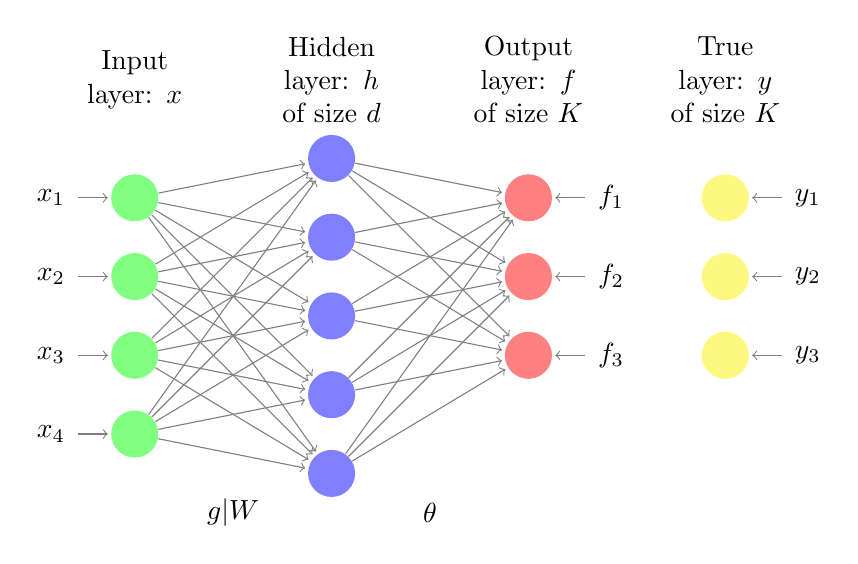
\begin{tikzpicture}[shorten >=1pt,->,draw=black!50, node distance=\layersep]
    \tikzstyle{every pin edge}=[<-,shorten <=1pt]
    \tikzstyle{neuron}=[circle,fill=black!25,minimum size=17pt,inner sep=0pt]
    \tikzstyle{input neuron}=[neuron, fill=green!50];
    \tikzstyle{output neuron}=[neuron, fill=red!50];
    \tikzstyle{hidden neuron}=[neuron, fill=blue!50];
    \tikzstyle{true neuron}=[neuron, fill=yellow!50];
    \tikzstyle{annot} = [text width=4em, text centered]

    % Draw the input layer nodes
    \foreach \name / \y in {1,...,4}
    % This is the same as writing \foreach \name / \y in {1/1,2/2,3/3,4/4}
        \node[input neuron, pin=left:$x_{\y}$ ] (I-\name) at (0,-\y) {};

    % Draw the hidden layer nodes
    \foreach \name / \y in {1,...,5}
        \path[yshift=0.5cm] node[hidden neuron] (H-\name) at (\layersep,-\y cm) {};

    % Draw the output layer node
    % \node[output neuron,pin={[pin edge={->}]right:Output}, right of=H-3] (O) {};

	\foreach \name / \y in {1,...,3}
        \node[output neuron, pin=right:$f_{\y}$ ] (O-\name) at (\layersep*2,-\y) {};

    % Draw the true layer node

	\foreach \name / \y in {1,...,3}
        \node[true neuron, pin=right:$y_{\y}$ ] (T-\name) at (\layersep*3,-\y) {};


    % Connect every node in the input layer with every node in the
    % hidden layer.
    \foreach \source in {1,...,4}
        \foreach \dest in {1,...,5}
            \path (I-\source) edge (H-\dest);

    % Connect every node in the hidden layer with the output layer
    \foreach \source in {1,...,5}
        \foreach \dest in {1,...,3}
	        \path (H-\source) edge (O-\dest);

    % Annotate the layers
    \node[annot,above of=H-1, node distance=1cm] (hl) {Hidden layer: $h$ of size $d$};
    \node[annot,left of=hl] {Input layer: $x$};
    \node[annot,right of=hl] (ol) {Output layer: $f$ of size $K$};
    \node[annot,right of=ol] {True layer: $y$ of size $K$};

    \node[annot] (W) at (\layersep/2,-5) {$g|W$};
    \node[annot] (W) at (\layersep*3/2,-5) {$\theta$};

\end{tikzpicture}

\subsubsection*{Gradient retropropagation}


\begin{align}
	\frac{ \partial E } { \partial f_k } = 
		\left\{
		    \begin{array}{ll}
		        - \frac{1}{f_k} & \mbox{if } y_k =1 \\
		        \frac{1}{1 - f_k} & \mbox{if } y_k =0
		    \end{array}
		\right.
\end{align}


\begin{align}
	\frac{ \partial E } { \partial s_k } 
		=  
		\frac{ \partial E } { \partial f_k } \cdot \frac{ \partial f_k } { \partial s_k } 
		&=
		\left\{
		    \begin{array}{ll}
		        - \frac{1}{f_k} \cdot f_k (1 - f_k)& \mbox{if } y_k =1 \\
		        \frac{1}{1 - f_k} \cdot f_k (1 - f_k)& \mbox{if } y_k =0
		    \end{array}
		\right. \\
		&=
		\left\{
		    \begin{array}{ll}
		       f_k - 1 & \mbox{if } y_k =1 \\
		       f_k & \mbox{if } y_k =0
		    \end{array}
		\right. \\
		&= f_k - y_k
\end{align}



\begin{align}
	\frac{\partial E}{\partial \theta_i^{(k)}} 
	= 
	\frac{\partial E}{\partial s_k} \cdot \frac{\partial s_k}{\partial \theta_i^{(k)}} 
	= 
	h_i (f_k - y_k)
\end{align}


Trick: derivate $E$ in regard to $s_k$:
\begin{align}
	\frac{\partial E}{\partial h_i} 
	&= 
	\sum_{k=1}^K \frac{\partial E}{\partial s_k} \cdot \frac{\partial s_k}{\partial h_i} \\
	&= 
	\sum_{k=1}^K \theta_i^{(k)} (f_k - y_k)
\end{align}

We now have the gradient of E in regard to the output of the hidden layer. The equation to update $W$ will depend of which $g$ is chosen.


%\cleardoublepage

%\bibliographystyle{plain}
%\bibliography{biblio}

\end{document}
